%Note one sentence in one text line.
\section{VPN Based Mobile Measurement Platform} 
\label{sec:platform} 
In this section, we enumerate the goals of a mobile measurement platform, show how VPNs can be used to achieve the described goals, and finally present empirical results that demonstrate the feasibility of \platname, a VPN based platform for mobile network traffic measurement.

\subsection{Goals}  
\label{sec:goals} 
The primary goal for our platform is to provide comprehensive visibility into mobile networking traffic. 
To meet this goal, we further identify the following sub-goals that address limitations of the existing platforms discussed in \fref{sec:motivation}.
\begin{packedenumerate}
\item \emph{Portable.} We want our solution to work regardless of operating system, access technology, and service provider. 
\item \emph{Pervasive.} For maximum transparency, our system should provide seamless visibility into all network traffic generated by devices. 
This means continuous monitoring over time and as users move with their 
\item \emph{Passive} For comprehensive and independent of user triggers we want our solution to passively perform measurements. 
\item \emph{Deployable.} Our solution should be easy to use, immediately deployable and incur reasonable costs (or none at all) for users.
Furthermore, it should not incur the cost of warranty-voiding the device and by relying on techniques such as rooting a phone.
\end{packedenumerate}    

\subsection{Description}
\label{sec:description}

We believe that VPNs can be used to setup a portable, pervasive, and deployable measurement platform for mobile device. 
Our motivation was the use of VPNs by executives ``on the move'' to securely connect to corporate servers with their mobile device. 
The use of VPNs by corporate clients gave us hints towards considering VPNs as portable and deployable platform.
Further investigation showed us that Mobile OSes expose features that can make them pervasive.  


\subsubsection{Mobile Devices}

All iOS devices (version 3.0 and above) come with a feature called ``VPN On-Demand''. 
\emph{VPN On-Demand} forces the iOS device to use VPN tunnels when connecting to a specified set of domains. 
We use this feature to enforce our iOS devices to use a VPN tunnel to connect to the Internet.

Android version 4.0 and above comes with native VPN support. 
Unlike iOS, Android does not offer an equivalent of \emph{VPN On-Demand}; however, Android provides an API that allows an user space app to manage VPN connections. 
We modify the open source StrongSwan VPN client~\cite{strongswanclient} to ensure that the VPN reconnects each time the preferred network changes (\eg, when a device switches from cellular to \wifi). 
As of Android 4.2, Android supports ``Always On'' VPN connections that uses VPNs to tunnel all the data traffic. 
\tbd{Text on Issues with Always ON}.

\subsubsection{VPN Server}
Strongswan, Openswan, and OpenVPN are some of the popular VPN daemons that can be used to manage VPN tunnels. 
We use Strongswan because it is open source and, to the best of our knowledge, it is the only open source solution that can use the IPsec services of the Linux kernel without any kernel modifications. 
IPsec is important because the \emph{VPN On-Demand} feature of iOS is supported only for VPN tunnels that use IPsec. 
Strongswan is supported on vanilla Linux operating systems which ensures that VPN tunnels can be managed using \emph{off-the-shelf} software and hardware.

In summary, the active use of VPNs to access corporate networks regardless of the ISP, access technology motivated us to consider VPNs. 
Mobile devices can connect to open source VPN implementation that can run on off-the-shelf servers. 
Our platform relies on VPNs to tunnel and capture the mobile data traffic. 
We use the open source Strongswan daemon to manage VPN tunnels. 
We use tcpdump to capture the packets on the server that runs Strongswan. 
Our servers have been deployed at the University of Washington and Inria and the mobile devices belong to users participating in an IRB-approved study. 

\tbd{How we capture and why this is important to label flows to access
technology and ISP?New instance of tcp dump for each flow. Each time a
tunnel is created separate instance of tcpdump used -- required to isolate
flows. We log the IP address from which tunnel is created. We use this IP
to get the details of the ISP. We then look up the ISP and label the
connection to be wifi or celluar. Pros and cons of this approach.}

\eat{
\begin{figure}
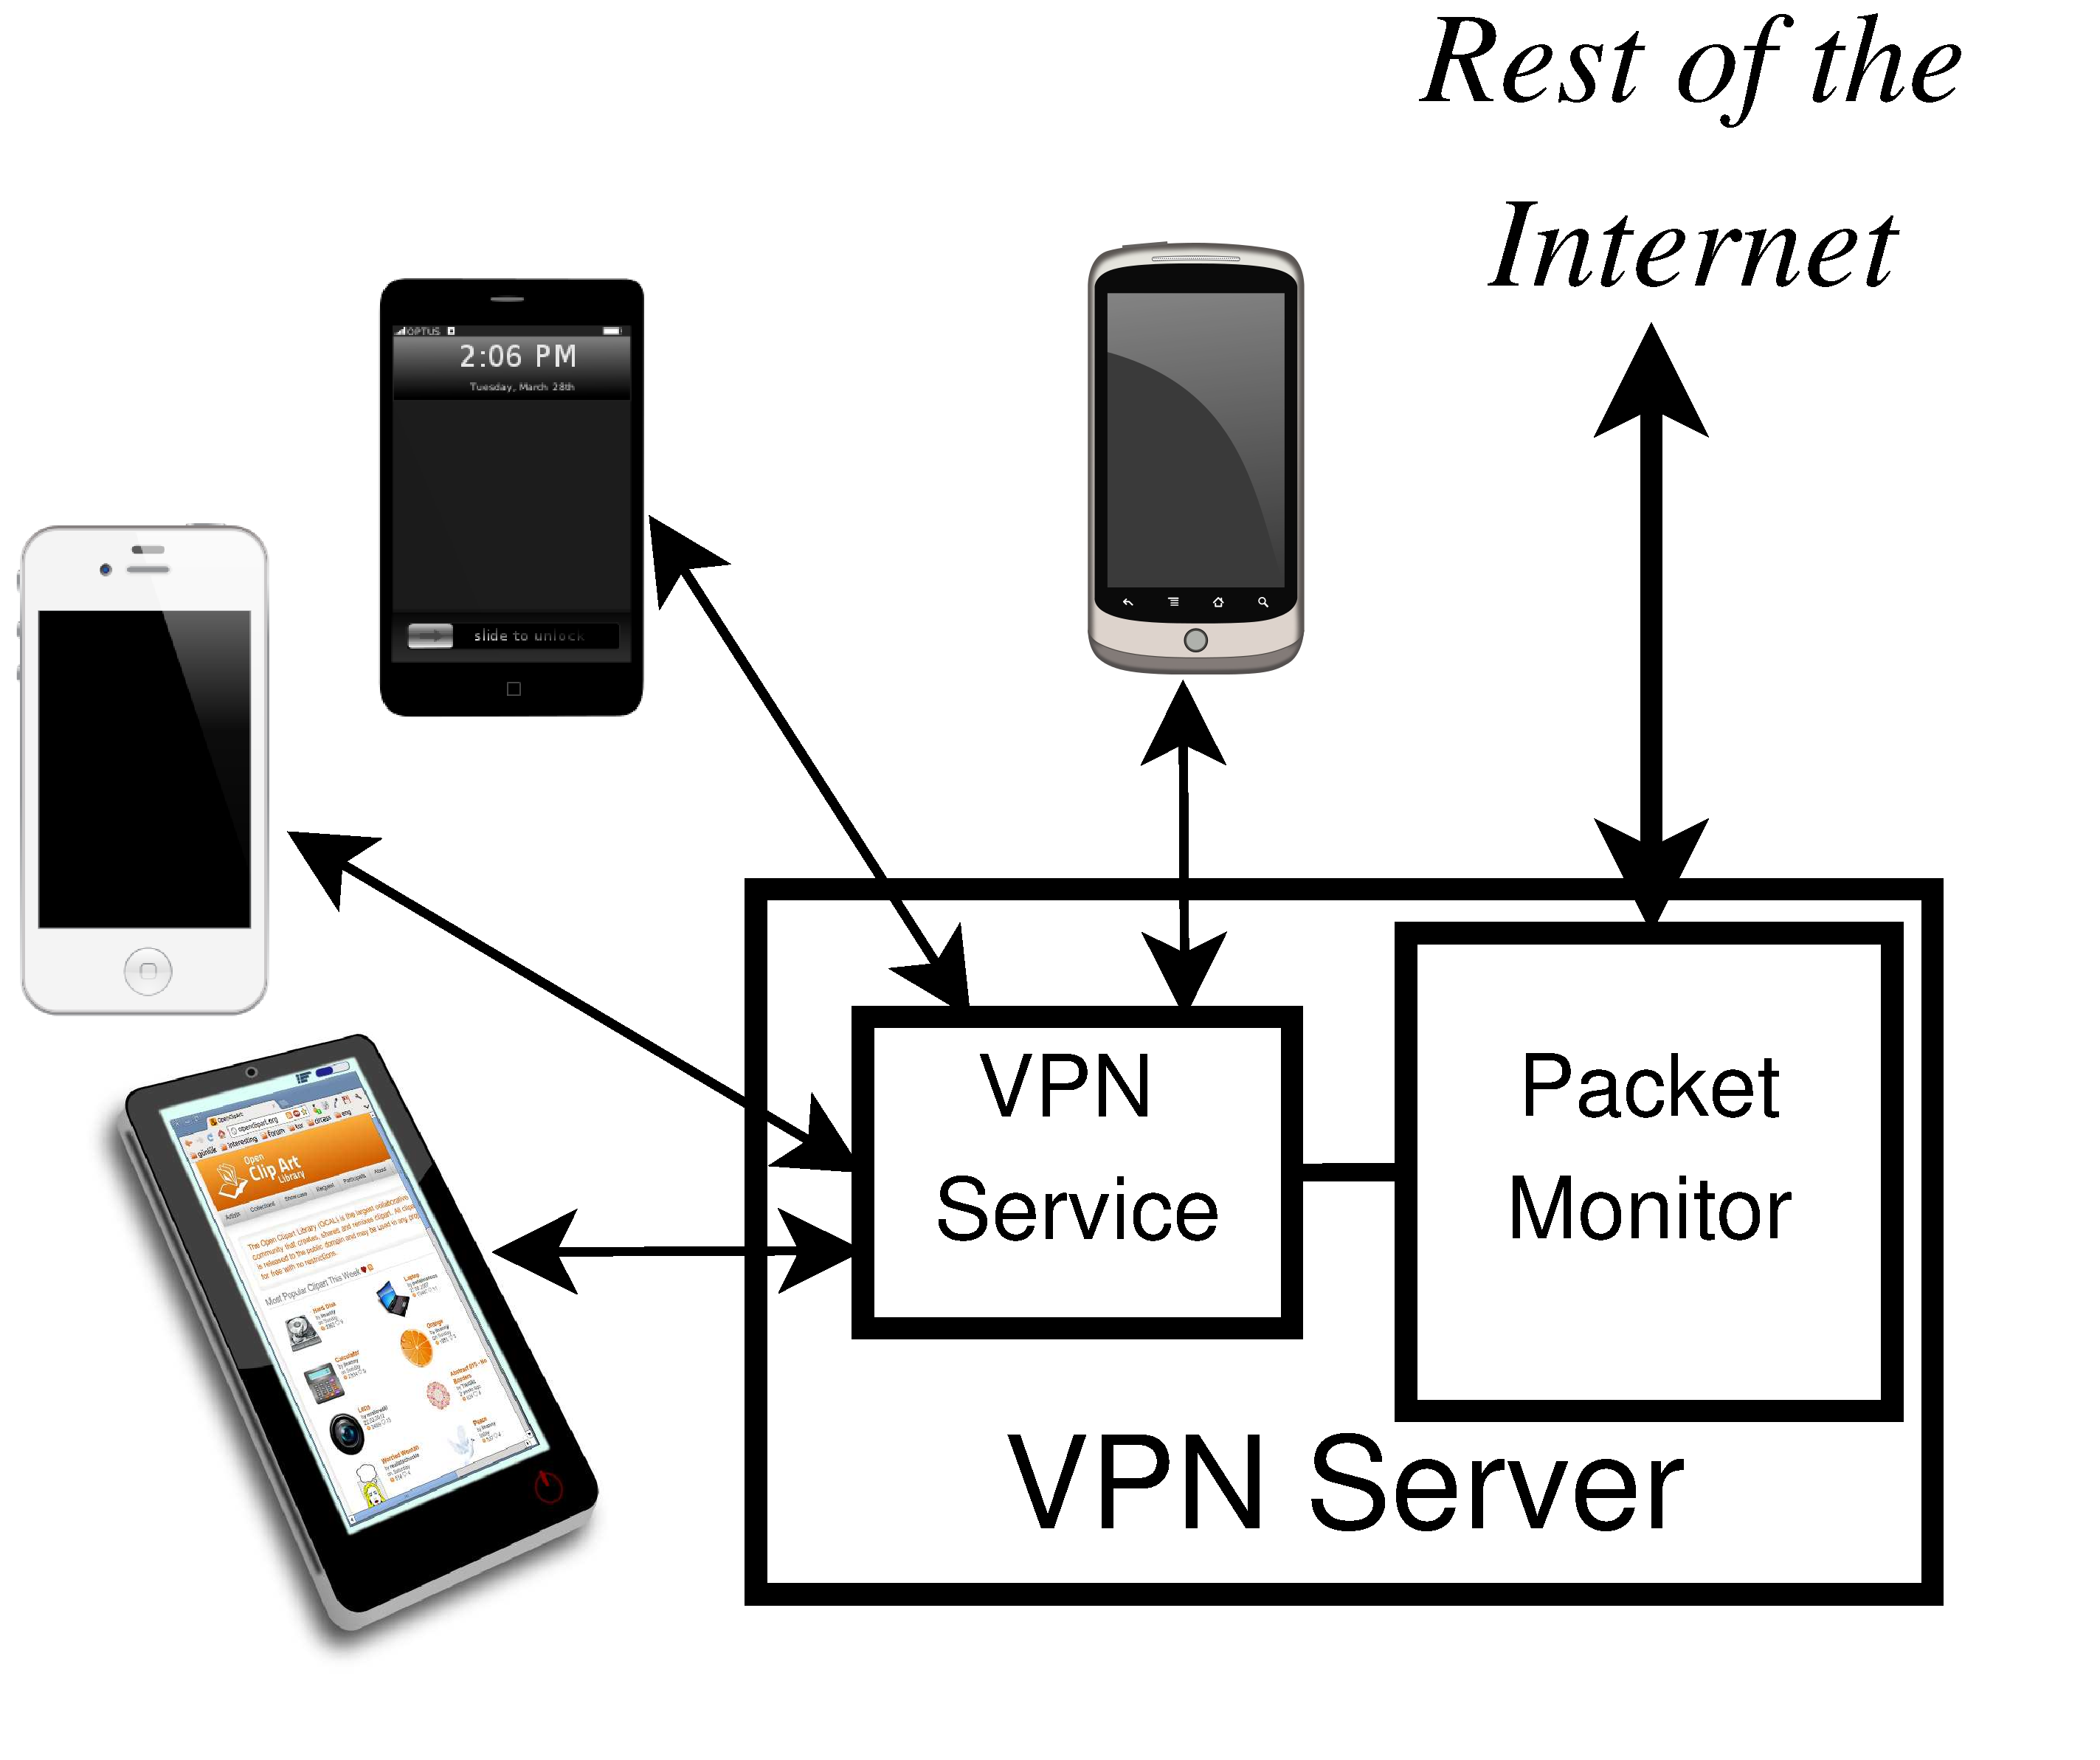
\includegraphics[width=0.75\columnwidth]{figures/meddle-servers.pdf}
\caption{\tbd{I am not sure if we need this figure}}
\label{fig:description}
\end{figure}
}

\subsection{Feasibility}

We now show that a VPN based platform is portable, pervasive, deployable, and incurs a small overhead in terms of latency, power, and bandwidth. 

\subsubsection{Portable, Pervasive, Passive, and Deployable} 
% device, access technology, and service provider. 
Android, BlackBerry, Bada, and iOS all support VPNs natively, representing more than 86\% of the mobile device market\cite{gartner-phone-share}. 
These devices support VPN tunnels over Wi-Fi and the cellular interface.
Furthermore, to satisfy their corporate clients, very few ISPs are known to block VPN traffic to flow through their networks.  

% devices connect seamlessly without periodic action.
We use the ``VPN On-Demand'' feature provided by iOS to ensure that our system is pervasive. 
Android provides an API that allows user space apps to manage VPN connections. 
We modify the open source StrongSwan VPN client~\cite{strongswanclient} to ensure that the VPN reconnects each time the preferred network changes (\eg, when a device switches from cellular to \wifi). 
As of Android 4.2, Android supports ``Always On'' VPN connections that uses VPNs to tunnel all the data traffic. 
\tbd{Text on Issues with Always ON}.

Manually configuring a VPN generally requires filling out five fields on an Android phone, and the VPN configuration can be distributed using a single file on iOS.
These configurations are primarily required to drive the key exchange algorithms that establish the VPN tunnels. 
This simplicity is important because it can facilitate realistic measurement studies with end users.  

In summary, native VPN support along with a set of features exposed to by mobile OSes to manage VPNs offer a solid foundation to build a portable, pervasive, passive, and deployable platform for mobile measurements.

\subsubsection{Latency Overheads}
Number of round trip times to establish the connection. 
\tbd{Text from results from Adrian and Sam}

\subsubsection{Power Overheads}
\tbd{TODO if needed}

\subsubsection{Bandwidth Overheads} 

Number of packets to establish the connection 

IPSec encapsulation slightly inflates packet sizes, in addition to preventing carrier middleboxes from applying their own compression. 
We measured the overhead of the tunnel in terms of data overhead from IPsec headers and keep-alive messages, finding that it ranges from \tbd{range}\%.

For our measurements, we capture the encrypted packets exchanged by our servers and the clients that use \platname. 
We performed the packet capture for \tbd{Number} days during which \tbd{number} devices tunneled their traffic via our  servers. 
During this time interval we also capture the packets that were encapsulated in the IPsec packets. 
We use these samples to compute the increase in the amount of bytes transferred due to encapsulation and the keep-alive messages. 
During the 14 day period we observe that the median of the increase to be \tbd{number}\%, with a maximum increase of \tbd{number}\%

\tbd{In Summary, ...}
